\section{Social Network}\label{sec:fa_social_network}

The current design for the escolinhas.pt social network is dynamic in nature, and extracted from the relationships formed through the connections between users and their roles with schools, groups, and even another roles, as depicted in Fig.~\ref{fig:social_network_current}. This allows the construction of a network where all the connections can be inferred dynamically and where an user can be identified another through their connections: friends, classmates, parent--child, teacher--student, and so on.

\begin{figure}[H]
  \centering
  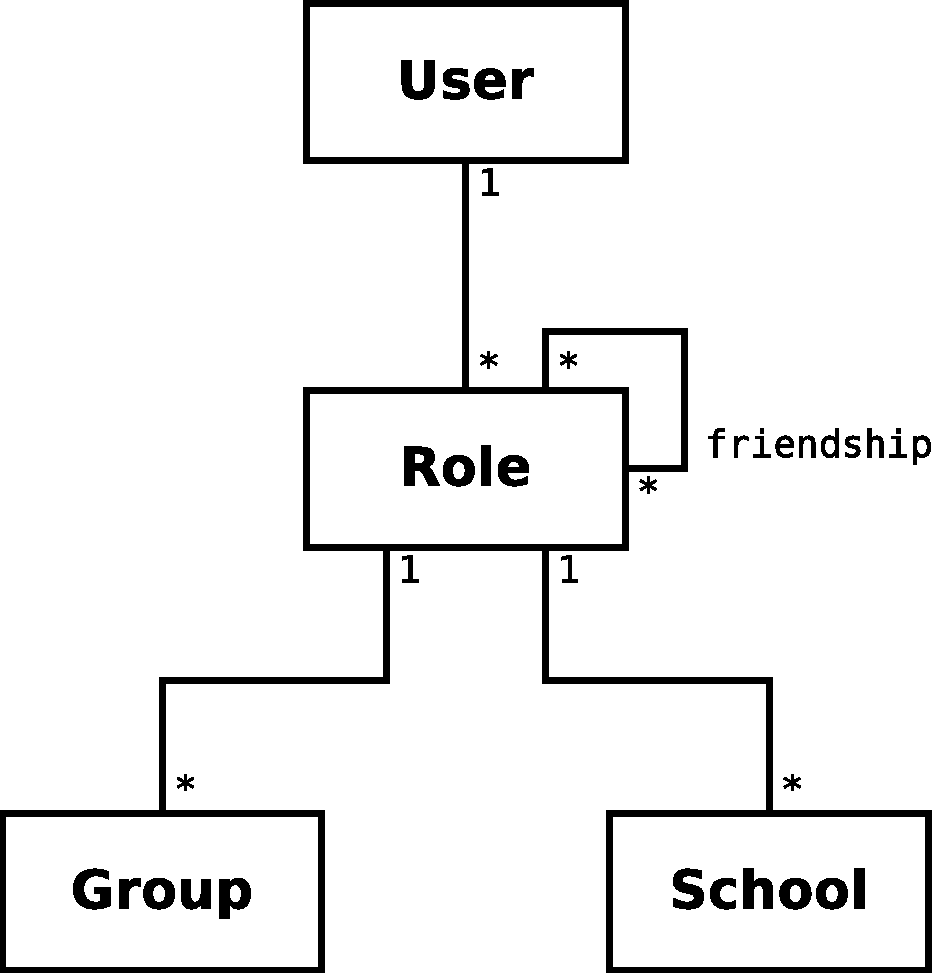
\includegraphics[width=65mm]{social_network_current.pdf}
  \caption{Current User Network Model}
  \label{fig:social_network_current}
\end{figure}

\subsection{Variability Requirements}\label{sec:fa_social_network_variability_requirements}

This model, however useful, offers a very small degree of variability. Due to the closed nature of the platform, there is a need to provide mechanisms able to fine-tune these connections in order to cater to each school specific needs. These mechanisms need to be available at the system administrator level, in order to easily manipulate these links without the need to pollute the application's codebase with hard-coded rules and without the need for redeployement.

\subsection{Candidate Patterns}\label{sec:fa_social_network_candidate_patterns}

Ideally, the user network would be described with a simple, self-referencing model, as shown in figure~\ref{fig:ideal_social_network_users}. This allows to create static relationships between any two users that can be edited as needed. This would work great if all that was needed was to create realtionships between users. However, it is often necessary to create connections between users and other entities in the system, such as groups and schools. Thus, this simple model needs to be abstracted in order to connect any two entities present in the system, whichever they may be, as shown in Fig.~\ref{fig:ideal_social_network_things}.

\begin{figure}[H]
  \centering
  \subfloat[Users Network]{\label{fig:ideal_social_network_users}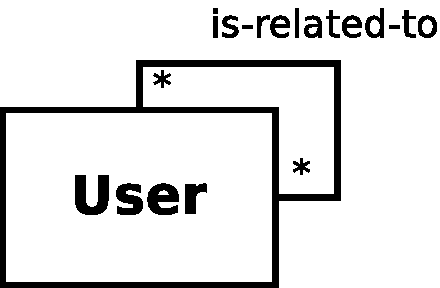
\includegraphics[width=25mm]{ideal_social_network_users}}
  \hspace{20mm}
  \subfloat[Entities Network]{\label{fig:ideal_social_network_things}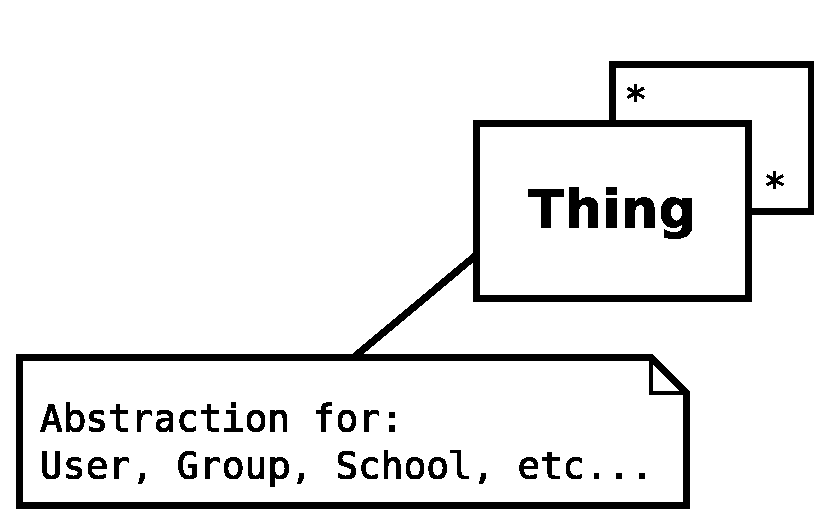
\includegraphics[width=55mm]{ideal_social_network_things}}
  \caption{Simplified Network Models}
  \label{fig:simplified_network_models}
\end{figure}

\subsection{Chosen Patterns \& Rationale}\label{sec:fa_social_network_chosen_patterns_rationale}

Despite solving the majority of the problem, the solutions described in \ref{fa_social_network_candidate_patterns} are less than ideal, as they do not allow the identification of an user before another, because only a direct connection between two different entities is contemplated. As such, for this particular problem, \textbf{?we?} need to be able to connect any two entities in the system, with an optional third entity to serve as hint as to how the original entities are connected. This problem can be solved by using the \textsc{Accountability} pattern (see \ref{sec:relationships_between_entities}) by Martin Fowler \cite{fowler_accountability}: it allows a bi-directional relationship between two entities (also known as \emph{parties}) while maintaining an AccountabilityType which can be used to store aditional data about the connection. As such, this AccountabilityType can be used to store an optional third party, responsible for identifying how the two other parties are connected --- effectivelly granting means to identify an user before an other, which is part of the original problem formulation (\ref{sec:fa_social_network}).

\subsection{Implementation}\label{sec:fa_social_network_implementation}

A variant of the \textsc{Accountability} design pattern was chosen (shown in Fig.~\ref{fig:social_network_conceptual}). This implementation follows the original description of the pattern by using all the usual entities present in the original \textsc{Accountability} pattern \cite{fowler_accountability} - however, it denormalizes the AccountabilityType entity \emph{into} the Accountabilities themselves. Despite creating some data redundancy, this option provides a more performant implementation: as the Accountabilities table is to be constantly accessed, the decision to have the AccountabilityTypes in a separate table would lead to expensive \verb!JOIN! operations. This, in turn, would lead to a less than desirable performance and complexity. \textbf{I PROBABLY NEED TO BACK THIS UP WITH SOME DATA!!!}

\begin{figure}[H]
  \centering
  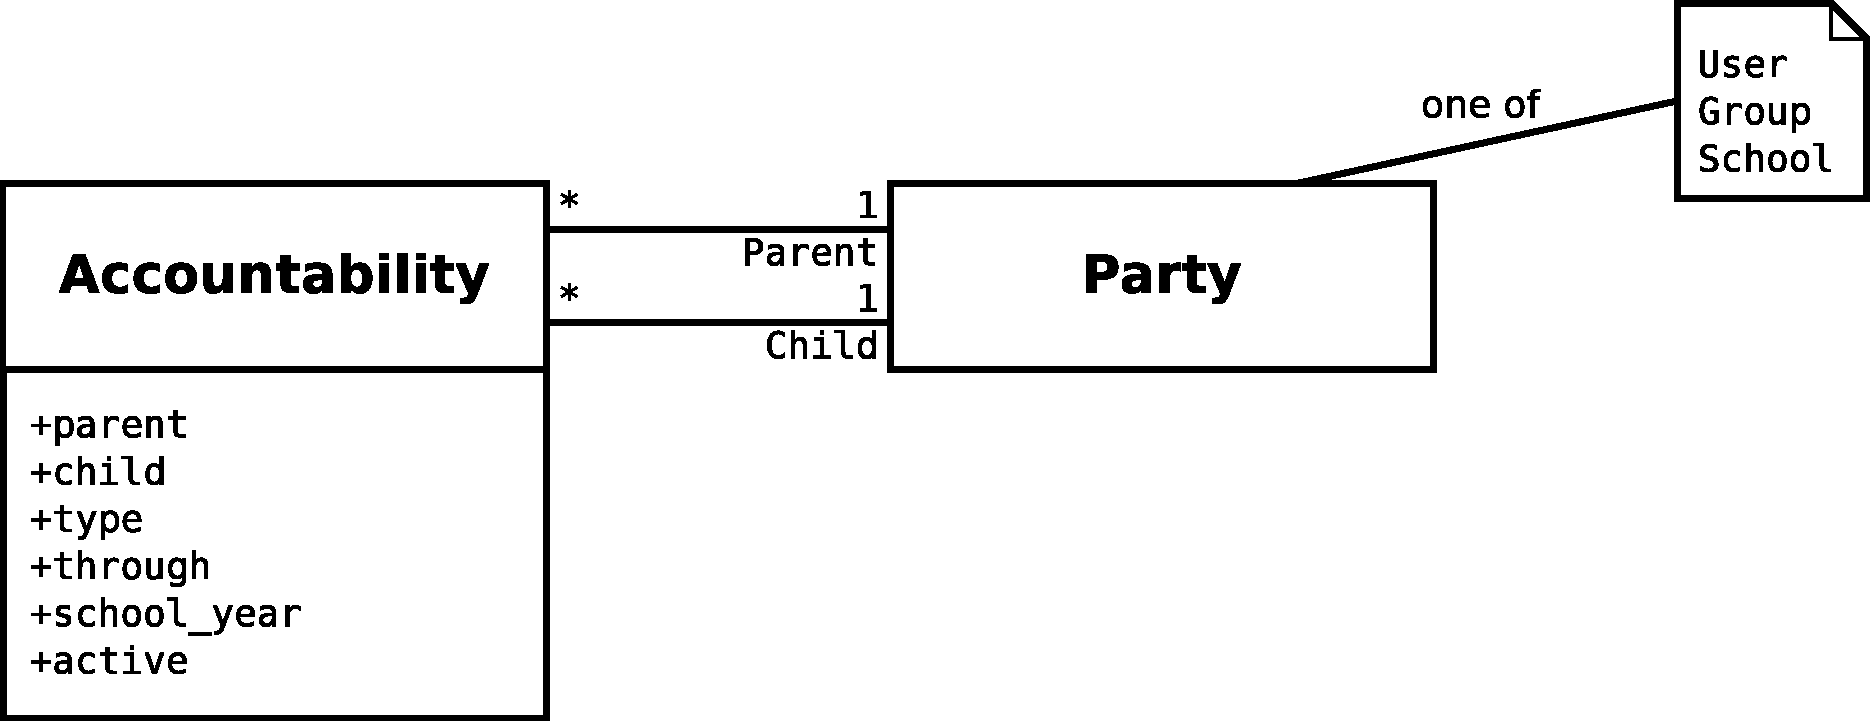
\includegraphics[width=115mm]{social_network_conceptual}
  \caption{Conceptual User Network Model}
  \label{fig:social_network_conceptual}
\end{figure}

\subsection{Impact Analysis}\label{sec:fa_social_network_impact_analysis}
